\documentclass{standalone}
\usepackage{pgfplots}
\pgfplotsset{width=7cm,compat=1.8}
\usepgfplotslibrary{fillbetween}

\usepackage{unicode-math}
\usepackage{siunitx}


\pgfdeclareverticalshading{heat}{3cm}{
rgb(0.013cm)=(0.001462,0.000466,0.013866);
rgb(0.027cm)=(0.003299,0.002249,0.024239);
rgb(0.040cm)=(0.006006,0.004692,0.038558);
rgb(0.053cm)=(0.009561,0.007713,0.055143);
rgb(0.066cm)=(0.013995,0.011225,0.071862);
rgb(0.080cm)=(0.019373,0.015133,0.088767);
rgb(0.093cm)=(0.025793,0.019331,0.10593);
rgb(0.106cm)=(0.033385,0.023702,0.123397);
rgb(0.120cm)=(0.042253,0.028139,0.141141);
rgb(0.133cm)=(0.051644,0.032474,0.159254);
rgb(0.146cm)=(0.06134,0.03659,0.177642);
rgb(0.159cm)=(0.071429,0.040294,0.196354);
rgb(0.173cm)=(0.081962,0.043328,0.215289);
rgb(0.186cm)=(0.09299,0.045583,0.234358);
rgb(0.199cm)=(0.104551,0.047008,0.25343);
rgb(0.212cm)=(0.116656,0.047574,0.272321);
rgb(0.226cm)=(0.129285,0.047293,0.290788);
rgb(0.239cm)=(0.142378,0.046242,0.308553);
rgb(0.252cm)=(0.15585,0.044559,0.325338);
rgb(0.266cm)=(0.169575,0.042489,0.340874);
rgb(0.279cm)=(0.183429,0.040329,0.354971);
rgb(0.292cm)=(0.197297,0.0384,0.367535);
rgb(0.305cm)=(0.211095,0.03703,0.378563);
rgb(0.319cm)=(0.224763,0.036405,0.388129);
rgb(0.332cm)=(0.238273,0.036621,0.396353);
rgb(0.345cm)=(0.25162,0.037705,0.403378);
rgb(0.359cm)=(0.26481,0.039647,0.409345);
rgb(0.372cm)=(0.27785,0.042353,0.414392);
rgb(0.385cm)=(0.290763,0.045644,0.418637);
rgb(0.398cm)=(0.303568,0.049396,0.422182);
rgb(0.412cm)=(0.316282,0.05349,0.425116);
rgb(0.425cm)=(0.328921,0.057827,0.427511);
rgb(0.438cm)=(0.3415,0.062325,0.429425);
rgb(0.452cm)=(0.354032,0.066925,0.430906);
rgb(0.465cm)=(0.366529,0.071579,0.431994);
rgb(0.478cm)=(0.379001,0.076253,0.432719);
rgb(0.491cm)=(0.391453,0.080927,0.433109);
rgb(0.505cm)=(0.403894,0.08558,0.433179);
rgb(0.518cm)=(0.416331,0.090203,0.432943);
rgb(0.531cm)=(0.428768,0.09479,0.432412);
rgb(0.545cm)=(0.441207,0.099338,0.431594);
rgb(0.558cm)=(0.453651,0.103848,0.430498);
rgb(0.571cm)=(0.4661,0.108322,0.429125);
rgb(0.584cm)=(0.478558,0.112764,0.427475);
rgb(0.598cm)=(0.491022,0.117179,0.425552);
rgb(0.611cm)=(0.503493,0.121575,0.423356);
rgb(0.624cm)=(0.515967,0.12596,0.420887);
rgb(0.637cm)=(0.528444,0.130341,0.418142);
rgb(0.651cm)=(0.54092,0.134729,0.415123);
rgb(0.664cm)=(0.553392,0.139134,0.411829);
rgb(0.677cm)=(0.565854,0.143567,0.408258);
rgb(0.691cm)=(0.578304,0.148039,0.404411);
rgb(0.704cm)=(0.590734,0.152563,0.40029);
rgb(0.717cm)=(0.603139,0.157151,0.395891);
rgb(0.730cm)=(0.615513,0.161817,0.391219);
rgb(0.744cm)=(0.627847,0.166575,0.386276);
rgb(0.757cm)=(0.640135,0.171438,0.381065);
rgb(0.770cm)=(0.652369,0.176421,0.375586);
rgb(0.784cm)=(0.66454,0.181539,0.369846);
rgb(0.797cm)=(0.676638,0.186807,0.363849);
rgb(0.810cm)=(0.688653,0.192239,0.357603);
rgb(0.823cm)=(0.700576,0.197851,0.351113);
rgb(0.837cm)=(0.712396,0.203656,0.344383);
rgb(0.850cm)=(0.724103,0.20967,0.337424);
rgb(0.863cm)=(0.735683,0.215906,0.330245);
rgb(0.877cm)=(0.747127,0.222378,0.322856);
rgb(0.890cm)=(0.758422,0.229097,0.315266);
rgb(0.903cm)=(0.769556,0.236077,0.307485);
rgb(0.916cm)=(0.780517,0.243327,0.299523);
rgb(0.930cm)=(0.791293,0.250856,0.29139);
rgb(0.943cm)=(0.801871,0.258674,0.283099);
rgb(0.956cm)=(0.812239,0.266786,0.274661);
rgb(0.970cm)=(0.822386,0.275197,0.266085);
rgb(0.983cm)=(0.832299,0.283913,0.257383);
rgb(0.996cm)=(0.841969,0.292933,0.248564);
rgb(1.009cm)=(0.851384,0.30226,0.239636);
rgb(1.023cm)=(0.860533,0.311892,0.230606);
rgb(1.036cm)=(0.869409,0.321827,0.221482);
rgb(1.049cm)=(0.878001,0.33206,0.212268);
rgb(1.063cm)=(0.886302,0.342586,0.202968);
rgb(1.076cm)=(0.894305,0.353399,0.193584);
rgb(1.089cm)=(0.902003,0.364492,0.184116);
rgb(1.102cm)=(0.90939,0.375856,0.174563);
rgb(1.116cm)=(0.916462,0.387481,0.164924);
rgb(1.129cm)=(0.923215,0.399359,0.155193);
rgb(1.142cm)=(0.929644,0.411479,0.145367);
rgb(1.155cm)=(0.935747,0.423831,0.13544);
rgb(1.169cm)=(0.941521,0.436405,0.125409);
rgb(1.182cm)=(0.946965,0.449191,0.115272);
rgb(1.195cm)=(0.952075,0.462178,0.105031);
rgb(1.209cm)=(0.956852,0.475356,0.094695);
rgb(1.222cm)=(0.961293,0.488716,0.084289);
rgb(1.235cm)=(0.965397,0.502249,0.073859);
rgb(1.248cm)=(0.969163,0.515946,0.063488);
rgb(1.262cm)=(0.97259,0.529798,0.053324);
rgb(1.275cm)=(0.975677,0.543798,0.043618);
rgb(1.288cm)=(0.978422,0.557937,0.034931);
rgb(1.302cm)=(0.980824,0.572209,0.028508);
rgb(1.315cm)=(0.982881,0.586606,0.024661);
rgb(1.328cm)=(0.984591,0.601122,0.023606);
rgb(1.341cm)=(0.985952,0.61575,0.025592);
rgb(1.355cm)=(0.986964,0.630485,0.030908);
rgb(1.368cm)=(0.987622,0.64532,0.039886);
rgb(1.381cm)=(0.987926,0.66025,0.05175);
rgb(1.395cm)=(0.987874,0.675267,0.065257);
rgb(1.408cm)=(0.987464,0.690366,0.07999);
rgb(1.421cm)=(0.986694,0.70554,0.095694);
rgb(1.434cm)=(0.985566,0.720782,0.112229);
rgb(1.448cm)=(0.984075,0.736087,0.129527);
rgb(1.461cm)=(0.982228,0.751442,0.147565);
rgb(1.474cm)=(0.980032,0.766837,0.166353);
rgb(1.488cm)=(0.977497,0.782258,0.185923);
rgb(1.501cm)=(0.974638,0.797692,0.206332);
rgb(1.514cm)=(0.971468,0.813122,0.227658);
rgb(1.527cm)=(0.968041,0.828515,0.249972);
rgb(1.541cm)=(0.964394,0.843848,0.273391);
rgb(1.554cm)=(0.960626,0.859069,0.29801);
rgb(1.567cm)=(0.956834,0.874129,0.323974);
rgb(1.580cm)=(0.953215,0.888942,0.351369);
rgb(1.594cm)=(0.950018,0.903409,0.380271);
rgb(1.607cm)=(0.947594,0.917399,0.410665);
rgb(1.620cm)=(0.946392,0.930761,0.442367);
rgb(1.634cm)=(0.946903,0.943348,0.47497);
rgb(1.647cm)=(0.949545,0.955063,0.50786);
rgb(1.660cm)=(0.954529,0.965896,0.540361);
rgb(1.673cm)=(0.961812,0.975924,0.571925);
rgb(1.687cm)=(0.971162,0.985282,0.602154);
rgb(1.700cm)=(0.982257,0.994109,0.631017)
}

\tikzset{
	WL/.style={
		prefix after command= {\pgfextra{\tikzset{every label/.style={
			white,
			label distance=4pt,
		}}}}
	}
}

\tikzset{
	every label/.style={
		label distance=4pt,
	}
}

\begin{document}

\pgfplotsset{set layers}


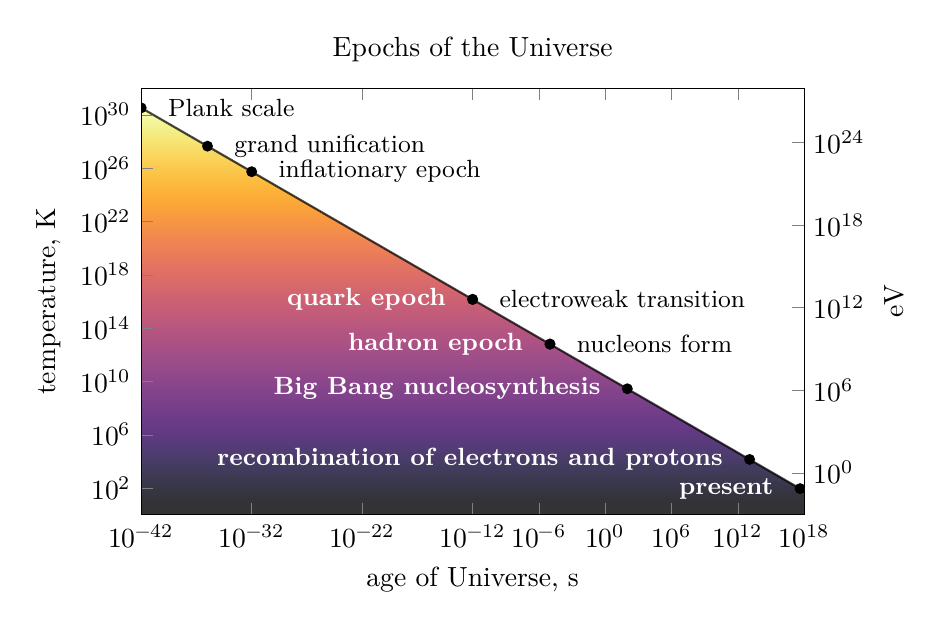
\begin{tikzpicture} 
	\begin{loglogaxis}[
		% scale=1.2,
		width=10cm,
		height=7cm,
		ymin=1, ymax=1e32,
		xmin=1e-42, xmax=1e18,
		xmin=1e-42, xmax=1e18,
		xlabel={age of Universe, \si{s}},
		ylabel={temperature, \si{K}},
		ytick={1e2,1e6,1e10,1e14,1e18,1e22,1e26,1e30},
		legend style={
			at={(0.9,0.1)},
			anchor=south east,
			legend cell align=right,
		},
		title={Epochs of the Universe},
		every axis plot/.append style={
			area legend,
			opacity=0.7,
		},
		every label/.style={
			label distance=1cm,
		},
		axis on top,
		ytick pos=left,
		xtick={1e18,1e12,1e6,1,1e-6,1e-12,1e-22,1e-32,1e-42},
	]
	\addplot[name path=t, thick] coordinates {
	(1e-43, 1e31)
	(1e18, 61)
	};

	\addplot[name path=axis] coordinates {
	(1e-42, 1)
	(1e19, 1)
	};


	\addplot[shading=heat, opacity=1] fill between [of=t and axis];
	\addplot[fill=white, opacity=0.2] fill between [of=t and axis];

	\node[label=right:{\small Plank scale}, fill, circle, inner sep=1.4pt] at (axis cs: 1e-42, 3.32e+30) {};
	\node[label=right:{\small grand unification}, fill, circle, inner sep=1.4pt] at (axis cs: 1e-36,4.45e+27) {};
	\node[label=right:{\small inflationary epoch}, fill, circle, inner sep=1.4pt] at (axis cs: 1e-32,5.4e+25) {};
	\node[label=right:{\small electroweak transition}, fill, circle, inner sep=1.4pt] at (axis cs: 1e-12,1.43e+16) {};
	\node[WL,label=left:{\small\bf quark epoch}, fill, circle, inner sep=1.4pt] at (axis cs: 1e-12,1.43e+16) {};
	\node[WL,label=left:{\small\bf hadron epoch}, fill, circle, inner sep=1.4pt] at (axis cs: 1e-05,6.36e+12) {};
	\node[label=right:{\small nucleons form}, fill, circle, inner sep=1.4pt] at (axis cs: 1e-05,6.36e+12) {};
	\node[WL,label=left:{\small\bf Big Bang nucleosynthesis}, fill, circle, inner sep=1.4pt] at (axis cs: 100,2.83e+09) {};
	\node[WL,label=left:{\small\bf recombination of electrons and protons}, fill, circle, inner sep=1.4pt] at (axis cs: 1.17e+13,1.42e+04) {};
	\node[WL,label=left:{\small\bf present}, fill, circle, inner sep=1.4pt] at (axis cs: 4.35e+17,91.8) {};
	\end{loglogaxis}

	\begin{loglogaxis}[
		width=10cm,
		height=7cm,
		axis y line*=right,
		xmin=1e-42, xmax=1e18,
		ymin=9e-4, ymax=8.6e27,
		ylabel={\si{\eV}},
		hide x axis,
		ytick pos=right,
		ytick={1, 1e6, 1e12, 1e18, 1e24},
		yticklabels={$10^0$,$10^6$,$10^{12}$,$10^{18}$,$10^{24}$,$10^{18}$$},
	]
	\end{loglogaxis}
\end{tikzpicture}  	

\end{document}
